\documentclass{beamer}
\usepackage[english]{babel}
\usepackage{geometry,amsmath,graphicx,stmaryrd,hyperref}
\geometry{landscape, letterpaper}

%%%%%%%%%% Start TeXmacs macros
\catcode`\<=\active \def<{
\fontencoding{T1}\selectfont\symbol{60}\fontencoding{\encodingdefault}}
\catcode`\>=\active \def>{
\fontencoding{T1}\selectfont\symbol{62}\fontencoding{\encodingdefault}}
\newcommand{\assign}{:=}
\newcommand{\colons}{\,:\,}
\newcommand{\tmem}[1]{{\em #1\/}}
\newcommand{\tmfnhomepage}[1]{\thanks{\textit{Web:} \texttt{#1}}}
\newcommand{\tmmathbf}[1]{\ensuremath{\boldsymbol{#1}}}
\newcommand{\tmop}[1]{\ensuremath{\operatorname{#1}}}
\newcommand{\tmstrong}[1]{\textbf{#1}}
\newcommand{\tmverbatim}[1]{\text{{\ttfamily{#1}}}}
%%%%%%%%%% End TeXmacs macros

\begin{document}

\title{Functional Programming}

\author{
  {\L}ukasz Stafiniak
  \tmfnhomepage{www.ii.uni.wroc.pl/\~{}lukstafi}
}

\institute{{\L}ukasz Stafiniak}

\maketitle

\title{Lecture 5: Polymorphism \& ADTs}

\subtitle{Parametric types. Abstract Data Types.\\
Example: maps using red-black trees.}

\maketitle

{\center{If you see any error on the slides, let me know!}}

{\newpage}

\section{Type Inference}

We have seen the rules that govern the assignment of types to expressions, but
how does OCaml guess what types to use, and when no correct types exist? It
solves equations.
\begin{itemize}
  \item Variables play two roles: of {\tmem{unknowns}} and of
  {\tmem{parameters}}.
  \begin{itemize}
    \item Inside:
    
    {\hlstd{\# }}{\hlkwa{let }}{\hlstd{f }}{\hlopt{=
    }}{\hlkwc{List}}{\hlopt{.}}{\hlstd{hd}}{\hlopt{;;}}{\hlendline{}}\\
    {\hlkwa{val }}{\hlstd{f }}{\hlopt{: }}{\hlstd{'a list }}{\hlopt{->
    }}{\hlstd{'a}}
    
    \tmverbatim{'a} is a parameter: it can become any type. Mathematically we
    write: $f : \forall \alpha . \alpha \tmop{list} \rightarrow \alpha$ -- the
    quantified type is called a {\tmem{type scheme}}.
    
    \item Inside:
    
    {\hlstd{\# }}{\hlkwa{let }}{\hlstd{x }}{\hlopt{= }}{\hlkwb{ref
    }}{\hlopt{[];;}}{\hlendline{}}\\
    {\hlkwa{val }}{\hlstd{x }}{\hlopt{: }}{\hlstd{'{\textunderscore}a list
    }}{\hlkwb{ref}}
    
    \tmverbatim{'\_a} is an unknown. It stands for a particular type like
    {\hlkwb{float}} \ or {\hlopt{(}}{\hlkwb{int }}{\hlopt{->
    }}{\hlkwb{int}}{\hlopt{)}}, OCaml just doesn't yet know the type.
    
    \item OCaml only reports unknowns like \tmverbatim{'\_a} in inferred types
    for reasons not relevant to functional programming. When unknowns appear
    in inferred type against our expectations, {\tmem{$\eta$-expansion}} may
    help: writing {\hlkwa{let }}{\hlstd{f x }}{\hlopt{= }}{\hlstd{expr x}}
    instead of {\hlkwa{let }}{\hlstd{f }}{\hlopt{= }}{\hlstd{expr}} -- for
    example:
    
    {\hlstd{\# }}{\hlkwa{let }}{\hlstd{f }}{\hlopt{=
    }}{\hlkwc{List}}{\hlopt{.}}{\hlstd{append }}{\hlopt{[];;}}{\hlendline{}}\\
    {\hlkwa{val }}{\hlstd{f }}{\hlopt{: }}{\hlstd{'{\textunderscore}a list
    }}{\hlopt{-> }}{\hlstd{'{\textunderscore}a list }}{\hlopt{=
    <}}{\hlkwa{fun}}{\hlopt{>}}{\hlendline{}}\\
    {\hlstd{\# }}{\hlkwa{let }}{\hlstd{f l }}{\hlopt{=
    }}{\hlkwc{List}}{\hlopt{.}}{\hlstd{append }}{\hlopt{[]
    }}{\hlstd{l}}{\hlopt{;;}}{\hlendline{}}\\
    {\hlkwa{val }}{\hlstd{f }}{\hlopt{: }}{\hlstd{'a list }}{\hlopt{->
    }}{\hlstd{'a list }}{\hlopt{= <}}{\hlkwa{fun}}{\hlopt{>}}
  \end{itemize}
  \item A {\tmem{type environment}} specifies what names (corresponding to
  parameters and definitions) are available for an expression, because they
  were introduced above it, and it specifies their types.
  
  \item Type inference solves equations over unknowns. ``What has to hold so
  that $e : \tau$ in type environment $\Gamma$?''
  \begin{itemize}
    \item If, for example, $f : \forall \alpha . \alpha \tmop{list}
    \rightarrow \alpha \in \Gamma$, then for $f : \tau$ we introduce $\gamma
    \tmop{list} \rightarrow \gamma = \tau$ for some fresh unknown $\gamma$.
    
    \item For $e_1 e_2 : \tau$ we introduce $\beta = \tau$ and ask for $e_1 :
    \gamma \rightarrow \beta$ and $e_2 : \gamma$, for some fresh unknowns
    $\beta, \gamma$.
    
    \item For $\tmop{fun} x \rightarrow e : \tau$ we introduce $\beta
    \rightarrow \gamma = \tau$ and ask for $e : \gamma$ in environment $\{ x :
    \beta \} \cup \Gamma$, for some fresh unknowns $\beta, \gamma$.
    
    \item Case $\tmop{let} x = e_1 \tmop{in} e_2 : \tau$ is different. One
    approach is to {\tmem{first}} solve the equations that we get by asking
    for $e_1 : \beta$, for some fresh unknown $\beta$. Let's say a solution
    $\beta = \tau_{\beta}$ has been found, $\alpha_1 \ldots \alpha_n \beta_1
    \ldots \beta_m$ are the remaining unknowns in $\tau_{\beta}$, \ and
    $\alpha_1 \ldots \alpha_n$ are all that do not appear in $\Gamma$. Then we
    ask for $e_2 : \tau$ in environment $\{ x : \forall \alpha_1 \ldots
    \alpha_n . \tau_{\beta} \} \cup \Gamma$.
    
    \item Remember that whenever we establish a solution $\beta =
    \tau_{\beta}$ to an unknown $\beta$, it takes effect everywhere!
    
    \item To find a type for $e$ (in environment $\Gamma$), we pick a fresh
    unknown $\beta$ and ask for $e : \beta$ (in $\Gamma$).
  \end{itemize}
  \item The ``top-level'' definitions for which the system infers types with
  variables are called {\tmem{polymorphic}}, which informally means ``working
  with different shapes of data''.
  \begin{itemize}
    \item This kind of polymorphism is called {\tmem{parametric
    polymorphism}}, since the types have parameters. A different kind of
    polymorphism is provided by object-oriented programming languages.
  \end{itemize}
\end{itemize}

\section{Parametric Types}

\begin{itemize}
  \item Polymorphic functions shine when used with polymorphic data types. In:
  
  {\hlkwa{type }}{\hlstd{'a my{\textunderscore}list }}{\hlopt{=
  }}{\hlkwd{Empty }}{\hlopt{\textbar }}{\hlkwd{Cons }}{\hlkwa{of }}{\hlstd{'a
  }}{\hlopt{* }}{\hlstd{'a my{\textunderscore}list}}
  
  we define lists that can store elements of any type \tmverbatim{'a}. Now:
  
  {\hlstd{\# }}{\hlkwa{let }}{\hlstd{tail l }}{\hlopt{=}}{\hlendline{}}\\
  {\hlstd{ \ }}{\hlkwa{match }}{\hlstd{l }}{\hlkwa{with}}{\hlendline{}}\\
  {\hlstd{ \ \ \ }}{\hlopt{\textbar }}{\hlkwd{Empty }}{\hlopt{->
  }}{\hlstd{invalid{\textunderscore}arg
  }}{\hlstr{"tail"}}{\hlstd{{\hlendline{}}\\
  \ \ \ }}{\hlopt{\textbar }}{\hlkwd{Cons
  }}{\hlopt{(}}{\hlstd{{\textunderscore}}}{\hlopt{, }}{\hlstd{tl}}{\hlopt{) ->
  }}{\hlstd{tl}}{\hlopt{;;}}{\hlendline{}}\\
  {\hlstd{ \ \ \ \ \ }}{\hlkwa{val }}{\hlstd{tail }}{\hlopt{: }}{\hlstd{'a
  my{\textunderscore}list }}{\hlopt{-> }}{\hlstd{'a my{\textunderscore}list}}
  
  is a polymorphic function: works for lists with elements of any type.
  
  \item A {\tmem{parametric type}} like {\hlstd{'a my{\textunderscore}list}}
  {\tmem{is not}} itself a data type but a family of data types:
  {\hlkwb{bool}}{\hlstd{ my{\textunderscore}list}}, {\hlkwb{int}}{\hlstd{
  my{\textunderscore}list}} etc. {\tmem{are}} different types.
  \begin{itemize}
    \item We say that the type {\hlkwb{int}}{\hlstd{ my{\textunderscore}list}}
    {\tmem{instantiates}} the parametric type {\hlstd{'a
    my{\textunderscore}list}}. 
  \end{itemize}
  \item In OCaml, the syntax is a bit confusing: type parameters precede type
  name. For example:
  
  {\hlkwa{type }}{\hlopt{(}}{\hlstd{'a}}{\hlopt{, }}{\hlstd{'b}}{\hlopt{)
  }}{\hlstd{choice }}{\hlopt{= }}{\hlkwd{Left }}{\hlkwa{of }}{\hlstd{'a
  {\hlopt{\textbar}} }}{\hlkwd{Right }}{\hlkwa{of }}{\hlstd{'b}}
  
  has two parameters. Mathematically we would write $\tmop{choice} (\alpha,
  \beta)$.
  \begin{itemize}
    \item Functions do not have to be polymorphic:
    
    {\hlstd{\# }}{\hlkwa{let }}{\hlstd{get{\textunderscore}int c
    }}{\hlopt{=}}{\hlendline{}}\\
    {\hlstd{ \ }}{\hlkwa{match }}{\hlstd{c }}{\hlkwa{with}}{\hlendline{}}\\
    {\hlstd{ \ \ \ }}{\hlopt{\textbar }}{\hlkwd{Left }}{\hlstd{i }}{\hlopt{->
    }}{\hlstd{i{\hlendline{}}\\
    \ \ \ }}{\hlopt{\textbar }}{\hlkwd{Right }}{\hlstd{b }}{\hlopt{->
    }}{\hlkwa{if }}{\hlstd{b }}{\hlkwa{then }}{\hlnum{1 }}{\hlkwa{else
    }}{\hlnum{0}}{\hlopt{;;}}{\hlendline{}}\\
    {\hlstd{ \ \ \ \ \ }}{\hlkwa{val }}{\hlstd{get{\textunderscore}int
    }}{\hlopt{: (}}{\hlkwb{int}}{\hlopt{, }}{\hlkwb{bool}}{\hlopt{)
    }}{\hlstd{choice }}{\hlopt{-> }}{\hlkwb{int}}
  \end{itemize}
  \item In F\#, we provide parameters (when more than one) after type name:
  
  {\hlkwa{type
  }}{\hlstd{choice}}{\hlopt{<}}\tmverbatim{'a,'}{\hlstd{b}}{\hlopt{> =
  }}{\hlkwd{Left }}{\hlkwa{of }}\tmverbatim{'a }{\hlopt{\textbar}}\tmverbatim{
  Right of }{\hlstd{'b}}
  
  \item In Haskell, we provide type parameters similarly to function
  arguments:
  
  {\hlkwd{data }}{\hlstd{Choice a b }}{\hlopt{= }}{\hlstd{Left a
  {\hlopt{\textbar}} Right b}}
\end{itemize}

\section{Type Inference, Formally}

\begin{itemize}
  \item A statement that an expression has a type in an environment is called
  a {\tmem{type judgement}}. For environment $\Gamma = \{ x : \forall \alpha_1
  \ldots \alpha_n . \tau_x ; \ldots \}$, expression $e$ and type $\tau$ we
  write
  \[ \Gamma \vdash e : \tau \]
  \item We will derive the equations in one go using $\llbracket \cdot
  \rrbracket$, to be solved later. Besides equations we will need to manage
  introduced variables, using existential quantification.
  
  \item For local definitions we require to remember what constraints should
  hold when the definition is used. Therefore we extend {\tmem{type schemes}}
  in the environment to: $\Gamma = \{ x : \forall \beta_1 \ldots \beta_m
  [\exists \alpha_1 \ldots \alpha_n .D] . \tau_x ; \ldots \}$ where $D$ are
  equations -- keeping the variables $\alpha_1 \ldots \alpha_n$ introduced
  while deriving $D$ in front.
  \begin{itemize}
    \item A simpler form would be enough: $\Gamma = \{ x : \forall \beta
    [\exists \alpha_1 \ldots \alpha_n .D] . \beta ; \ldots \}$
  \end{itemize}
\end{itemize}

\begin{eqnarray*}
  \llbracket \Gamma \vdash x : \tau \rrbracket & = & \exists \overline{\beta'}
  \bar{\alpha}' . (D [\bar{\beta} \bar{\alpha} \assign \overline{\beta'}
  \bar{\alpha}'] \wedge \tau_x [\bar{\beta} \bar{\alpha} \assign
  \overline{\beta'} \bar{\alpha}'] \dot{=} \tau)\\
  &  & \text{where } \Gamma (x) = \forall \bar{\beta} [\exists \bar{\alpha}
  .D] . \tau_x, \overline{\beta'} \bar{\alpha}' \# \tmop{FV} (\Gamma, \tau)\\
  &  & \\
  \left\llbracket \Gamma \vdash \tmmathbf{\tmop{fun}} x \text{\tmverbatim{->}}
  e : \tau \right\rrbracket & = & \exists \alpha_1 \alpha_2 . (\llbracket
  \Gamma \{ x : \alpha_1 \} \vdash e : \alpha_2 \rrbracket \wedge \alpha_1
  \rightarrow \alpha_2 \dot{=} \tau),\\
  &  & \text{where } \alpha_1 \alpha_2 \# \tmop{FV} (\Gamma, \tau)\\
  &  & \\
  \llbracket \Gamma \vdash e_1 e_2 : \tau \rrbracket & = & \exists \alpha .
  (\llbracket \Gamma \vdash e_1 : \alpha \rightarrow \tau \rrbracket \wedge
  \llbracket \Gamma \vdash e_2 : \alpha \rrbracket), \alpha \# \tmop{FV}
  (\Gamma, \tau)\\
  &  & \\
  \llbracket \Gamma \vdash K e_1 \ldots e_n : \tau \rrbracket & = & \exists
  \bar{\alpha}' . (\wedge_i \llbracket \Gamma \vdash e_i : \tau_i
  [\bar{\alpha} \assign \bar{\alpha}'] \rrbracket \wedge \varepsilon
  (\bar{\alpha}') \dot{=} \tau),\\
  &  & \text{w. } K \colons \forall \bar{\alpha} . \tau_1 \times \ldots
  \times \tau_n \rightarrow \varepsilon (\bar{\alpha}), \bar{\alpha}' \#
  \tmop{FV} (\Gamma, \tau)\\
  &  & \\
  \llbracket \Gamma \vdash e : \tau \rrbracket & = & (\exists \beta .C) \wedge
  \llbracket \Gamma \{x : \forall \beta [C] . \beta\} \vdash e_2 : \tau
  \rrbracket\\
  e = \tmmathbf{\tmop{let}} x = e_1 \tmmathbf{\tmop{in}} e_2 &  & \text{where
  } C = \llbracket \Gamma \vdash e_1 : \beta \rrbracket\\
  &  & \\
  \llbracket \Gamma \vdash e : \tau \rrbracket & = & (\exists \beta .C) \wedge
  \llbracket \Gamma \{x : \forall \beta [C] . \beta\} \vdash e_2 : \tau
  \rrbracket\\
  e = \tmmathbf{\tmop{letrec}} x = e_1 \tmmathbf{\tmop{in}} e_2 &  &
  \text{where } C = \llbracket \Gamma \{x : \beta\} \vdash e_1 : \beta
  \rrbracket\\
  &  & \\
  \llbracket \Gamma \vdash e : \tau \rrbracket & = & \exists \alpha_v .
  \llbracket \Gamma \vdash e_v : \alpha_v \rrbracket \wedge_i \llbracket
  \Gamma \vdash p_i .e_i : \alpha_v \rightarrow \tau \rrbracket,\\
  e = \tmmathbf{\tmop{match}} e_v \tmmathbf{\tmop{with}} \bar{c} &  & \alpha_v
  \# \tmop{FV} (\Gamma, \tau)\\
  \bar{c} = p_1 .e_1 | \ldots |p_n .e_n &  & \\
  &  & \\
  \llbracket \Gamma, \Sigma \vdash p.e : \tau_1 \rightarrow \tau_2 \rrbracket
  & = & \llbracket \Sigma \vdash p \downarrow \tau_1 \rrbracket \wedge \exists
  \bar{\beta} . \llbracket \Gamma \Gamma' \vdash e : \tau_2 \rrbracket\\
  &  & \text{where } \exists \bar{\beta} \Gamma' \text{ is } \llbracket
  \Sigma \vdash p \uparrow \tau_1 \rrbracket, \bar{\beta} \# \tmop{FV}
  (\Gamma, \tau_2)\\
  &  & \\
  \llbracket \Sigma \vdash p \downarrow \tau_1 \rrbracket &  & \text{derives
  constraints on type of matched value}\\
  &  & \\
  \llbracket \Sigma \vdash p \uparrow \tau_1 \rrbracket &  & \text{derives
  environment for pattern variables}
\end{eqnarray*}
\begin{itemize}
  \item By $\bar{\alpha}$ or $\overline{\alpha_i}$ we denote a sequence of
  some length: $\alpha_1 \ldots \alpha_n$
  
  \item By $\wedge_i \varphi_i$ we denote a conjunction of
  $\overline{\varphi_i}$: $\varphi_1 \ldots \varphi_n$.
\end{itemize}

\subsection{Polymorphic Recursion}

\begin{itemize}
  \item Note the limited polymorphism of {\hlkwa{let rec }}{\hlstd{f
  }}{\hlopt{=}} ... -- we cannot use \tmverbatim{f} polymorphically in its
  definition.
  \begin{itemize}
    \item In modern OCaml we can bypass the problem if we provide type of
    \tmverbatim{f} upfront: {\hlkwa{let rec }}{\hlstd{f }}{\hlopt{:
    }}{\hlstd{'a}}{\hlopt{. }}{\hlstd{'a }}{\hlopt{-> }}{\hlstd{'a
    list}}{\hlopt{ =}} ...
    
    \item where {\hlstd{'a}}{\hlopt{. }}{\hlstd{'a }}{\hlopt{-> }}{\hlstd{'a
    list}} stands for $\forall \alpha . \alpha \rightarrow \alpha
    \tmop{list}$.
  \end{itemize}
  \item Using the recursively defined function with different types in its
  definition is called polymorphic recursion.
  
  \item It is most useful together with irregular recursive datatypes where
  the recursive use has different type arguments than the actual parameters.
\end{itemize}

\subsubsection{Polymorphic Rec: A list alternating between two types of
elements}

{\hlkwa{type }}{\hlopt{(}}{\hlstd{'x}}{\hlopt{, '}}{\hlstd{o}}{\hlopt{)
}}{\hlstd{alterning }}{\hlopt{=}}{\hlendline{}}\\
{\hlopt{\textbar }}{\hlkwd{Stop}}{\hlendline{}}\\
{\hlopt{\textbar }}{\hlkwd{One }}{\hlkwa{of }}{\hlstd{'x }}{\hlopt{*
(}}{\hlstd{'o}}{\hlopt{, }}{\hlstd{'x}}{\hlopt{)
}}{\hlstd{alterning}}{\hlendline{}}\\
{\hlendline{}}\\
{\hlkwa{let rec }}{\hlstd{to{\textunderscore}list
}}{\hlopt{:}}{\hlendline{}}\\
{\hlstd{ \ \ \ 'x 'o 'a}}{\hlopt{.
(}}{\hlstd{'x}}{\hlopt{->}}{\hlstd{'a}}{\hlopt{) ->
(}}{\hlstd{'o}}{\hlopt{->}}{\hlstd{'a}}{\hlopt{) ->}}{\hlendline{}}\\
{\hlstd{ \ \ \ \ \ \ \ \ \ \ }}{\hlopt{(}}{\hlstd{'x}}{\hlopt{,
}}{\hlstd{'o}}{\hlopt{) }}{\hlstd{alterning }}{\hlopt{-> }}{\hlstd{'a list
}}{\hlopt{=}}{\hlendline{}}\\
{\hlstd{ \ }}{\hlkwa{fun }}{\hlstd{x2a o2a }}{\hlopt{->}}{\hlendline{}}\\
{\hlstd{ \ \ \ }}{\hlkwa{function}}{\hlendline{}}\\
{\hlstd{ \ \ \ }}{\hlopt{\textbar }}{\hlkwd{Stop }}{\hlopt{->
[]}}{\hlendline{}}\\
{\hlstd{ \ \ \ }}{\hlopt{\textbar }}{\hlkwd{One
}}{\hlopt{(}}{\hlstd{x}}{\hlopt{, }}{\hlstd{rest}}{\hlopt{) -> }}{\hlstd{x2a
x}}{\hlopt{::}}{\hlstd{to{\textunderscore}list o2a x2a rest}}{\hlendline{}}\\
{\hlendline{}}\\
{\hlkwa{let }}{\hlstd{to{\textunderscore}choice{\textunderscore}list alt
}}{\hlopt{=}}{\hlendline{}}\\
{\hlstd{ \ to{\textunderscore}list }}{\hlopt{(}}{\hlkwa{fun
}}{\hlstd{x}}{\hlopt{->}}{\hlkwd{Left }}{\hlstd{x}}{\hlopt{) (}}{\hlkwa{fun
}}{\hlstd{o}}{\hlopt{->}}{\hlkwd{Right }}{\hlstd{o}}{\hlopt{)
}}{\hlstd{alt}}{\hlendline{}}\\
{\hlendline{}}\\
{\hlkwa{let }}{\hlstd{it }}{\hlopt{=
}}{\hlstd{to{\textunderscore}choice{\textunderscore}list{\hlendline{}}\\
\ }}{\hlopt{(}}{\hlkwd{One }}{\hlopt{(}}{\hlnum{1}}{\hlopt{, }}{\hlkwd{One
}}{\hlopt{(}}{\hlstr{"o"}}{\hlopt{, }}{\hlkwd{One
}}{\hlopt{(}}{\hlnum{2}}{\hlopt{, }}{\hlkwd{One
}}{\hlopt{(}}{\hlstr{"oo"}}{\hlopt{,
}}{\hlkwd{Stop}}{\hlopt{)))))}}{\hlendline{}}\\


\subsubsection{Polymorphic Rec: Data-Structural Bootstrapping}

{\small{{\hlkwa{type }}{\hlstd{'a seq }}{\hlopt{= }}{\hlkwd{Nil
}}{\hlopt{\textbar }}{\hlkwd{Zero }}{\hlkwa{of }}{\hlopt{(}}{\hlstd{'a
}}{\hlopt{* }}{\hlstd{'a}}{\hlopt{) }}{\hlstd{seq {\hlopt{\textbar}}
}}{\hlkwd{One }}{\hlkwa{of }}{\hlstd{'a }}{\hlopt{* (}}{\hlstd{'a }}{\hlopt{*
}}{\hlstd{'a}}{\hlopt{) }}{\hlstd{seq}}{\hlendline{}}\\
{\hlendline{We store a list of elements in exponentially increasing
chunks.}}\\
{\hlkwa{let }}{\hlstd{example }}{\hlopt{=}}{\hlendline{}}\\
{\hlstd{ \ }}{\hlkwd{One }}{\hlopt{(}}{\hlnum{0}}{\hlopt{, }}{\hlkwd{One
}}{\hlopt{((}}{\hlnum{1}}{\hlopt{,}}{\hlnum{2}}{\hlopt{), }}{\hlkwd{Zero
}}{\hlopt{(}}{\hlkwd{One
}}{\hlopt{((((}}{\hlnum{3}}{\hlopt{,}}{\hlnum{4}}{\hlopt{),(}}{\hlnum{5}}{\hlopt{,}}{\hlnum{6}}{\hlopt{)),
((}}{\hlnum{7}}{\hlopt{,}}{\hlnum{8}}{\hlopt{),(}}{\hlnum{9}}{\hlopt{,}}{\hlnum{10}}{\hlopt{))),
}}{\hlkwd{Nil}}{\hlopt{))))}}{\hlendline{}}\\
{\hlendline{}}\\
{\hlkwa{let rec }}{\hlstd{cons }}{\hlopt{: }}{\hlstd{'a}}{\hlopt{.
}}{\hlstd{'a }}{\hlopt{-> }}{\hlstd{'a seq }}{\hlopt{-> }}{\hlstd{'a seq
}}{\hlopt{=}}{\hlendline{}}\\
{\hlstd{ \ }}{\hlkwa{fun }}{\hlstd{x }}{\hlopt{->
}}{\hlkwa{function}}{\hlendline{Appending an element to the datastructure is
like}}\\
{\hlstd{ \ }}{\hlopt{\textbar }}{\hlkwd{Nil }}{\hlopt{-> }}{\hlkwd{One
}}{\hlopt{(}}{\hlstd{x}}{\hlopt{, }}{\hlkwd{Nil}}{\hlopt{)}}{\hlendline{adding
one to a binary number: 1+0=1}}\\
{\hlstd{ \ }}{\hlopt{\textbar }}{\hlkwd{Zero }}{\hlstd{ps }}{\hlopt{->
}}{\hlkwd{One }}{\hlopt{(}}{\hlstd{x}}{\hlopt{,
}}{\hlstd{ps}}{\hlopt{)}}{\hlendline{1+...0=...1}}\\
{\hlstd{ \ }}{\hlopt{\textbar }}{\hlkwd{One }}{\hlopt{(}}{\hlstd{y}}{\hlopt{,
}}{\hlstd{ps}}{\hlopt{) -> }}{\hlkwd{Zero }}{\hlopt{(}}{\hlstd{cons
}}{\hlopt{(}}{\hlstd{x}}{\hlopt{,}}{\hlstd{y}}{\hlopt{)
}}{\hlstd{ps}}{\hlopt{)}}{\hlendline{1+...1=[...+1]0}}\\
{\hlendline{}}\\
{\hlkwa{let rec }}{\hlstd{lookup }}{\hlopt{: }}{\hlstd{'a}}{\hlopt{.
}}{\hlkwb{int }}{\hlopt{-> }}{\hlstd{'a seq }}{\hlopt{-> }}{\hlstd{'a
}}{\hlopt{=}}{\hlendline{}}\\
{\hlstd{ \ }}{\hlkwa{fun }}{\hlstd{i s }}{\hlopt{-> }}{\hlkwa{match
}}{\hlstd{i}}{\hlopt{, }}{\hlstd{s }}{\hlkwa{with}}{\hlendline{Rather than
returning \tmverbatim{None : 'a option}}}\\
{\hlstd{ \ {\hlopt{\textbar}} {\textunderscore}}}{\hlopt{, }}{\hlkwd{Nil
}}{\hlopt{-> }}{\hlstd{raise
}}{\hlkwd{Not{\textunderscore}found}}{\hlendline{we raise exception, for
convenience.}}\\
{\hlstd{ \ }}{\hlopt{\textbar }}{\hlnum{0}}{\hlopt{, }}{\hlkwd{One
}}{\hlopt{(}}{\hlstd{x}}{\hlopt{, }}{\hlstd{{\textunderscore}}}{\hlopt{) ->
}}{\hlstd{x{\hlendline{}}\\
\ {\hlopt{\textbar}} i}}{\hlopt{, }}{\hlkwd{One
}}{\hlopt{(}}{\hlstd{{\textunderscore}}}{\hlopt{, }}{\hlstd{ps}}{\hlopt{) ->
}}{\hlstd{lookup }}{\hlopt{(}}{\hlstd{i}}{\hlopt{-}}{\hlnum{1}}{\hlopt{)
(}}{\hlkwd{Zero }}{\hlstd{ps}}{\hlopt{)}}{\hlendline{}}\\
{\hlstd{ \ {\hlopt{\textbar}} i}}{\hlopt{, }}{\hlkwd{Zero }}{\hlstd{ps
}}{\hlopt{->}}{\hlendline{Random-Access lookup works}}\\
{\hlstd{ \ \ \ }}{\hlkwa{let }}{\hlstd{x}}{\hlopt{, }}{\hlstd{y }}{\hlopt{=
}}{\hlstd{lookup }}{\hlopt{(}}{\hlstd{i }}{\hlopt{/ }}{\hlnum{2}}{\hlopt{)
}}{\hlstd{ps }}{\hlkwa{in}}{\hlendline{in logarithmic time -- much faster
than}}\\
{\hlstd{ \ \ \ }}{\hlkwa{if }}{\hlstd{i }}{\hlkwa{mod }}{\hlnum{2 }}{\hlopt{=
}}{\hlnum{0 }}{\hlkwa{then }}{\hlstd{x }}{\hlkwa{else
}}{\hlstd{y}}{\hlendline{in standard lists.}}\\
}}

\section{Algebraic Specification}

\begin{itemize}
  \item The way we introduce a data structure, like complex numbers or
  strings, in mathematics, is by specifying an {\tmem{algebraic structure}}.
  
  \item Algebraic structures consist of a set (or several sets, for so-called
  {\tmem{multisorted}} algebras) and a bunch of functions (aka. operations)
  over this set (or sets).
  
  \item A {\tmem{signature}} is a rough description of an algebraic structure:
  it provides sorts -- names for the sets (in multisorted case) and names of
  the functions-operations together with their arity (and what sorts of
  arguments they take).
  
  \item We select a class of algebraic structures by providing axioms that
  have to hold. We will call such classes {\tmem{algebraic specifications}}.
  \begin{itemize}
    \item In mathematics, a rusty name for some algebraic specifications is a
    {\tmem{variety}}, a more modern and name is {\tmem{algebraic category}}.
  \end{itemize}
  \item Algebraic structures correspond to ``implementations'' and signatures
  to ``interfaces'' in programming languages.
  
  \item We will say that an algebraic structure implements an algebraic
  specification when all axioms of the specification hold in the structure.
  
  \item All algebraic specifications are implemented by multiple structures!
  
  \item We say that an algebraic structure does not have junk, when all its
  elements (i.e. elements in the sets corresponding to sorts) can be built
  using operations in its signature.
  
  \item We allow parametric types as sorts. {\small{In that case, strictly
  speaking, we define a family of algebraic specifications (a different
  specification for each instantiation of the parametric type).}}
\end{itemize}

\subsection{Algebraic specifications: examples}

\begin{itemize}
  \item An algebraic specification can also use an earlier specification.
  
  \item In ``impure'' languages like OCaml and F\# we allow that the result of
  any operation be an $\tmop{error}$. In Haskell we could use
  \tmverbatim{Maybe}.
\end{itemize}
\begin{tabular}{|l|}
  \hline
  $\tmop{nat}_p$\\
  \hline
  \begin{tabular}{l}
    $0 : \tmop{nat}_p$\\
    $\tmop{succ} : \tmop{nat}_p \rightarrow \tmop{nat}_p$\\
    $+ : \tmop{nat}_p \rightarrow \tmop{nat}_p \rightarrow \tmop{nat}_p$\\
    $\ast : \tmop{nat}_p \rightarrow \tmop{nat}_p \rightarrow \tmop{nat}_p$
  \end{tabular}\\
  \hline
  $n, m : \tmop{nat}_p$\\
  \hline
  \begin{tabular}{l}
    $0 + n = n$, $n + 0 = n$\\
    $m + \tmop{succ} (n) = \tmop{succ} (m + n)$\\
    $0 \ast n = 0$, $n \ast 0 = 0$\\
    $m \ast \tmop{succ} (n) = m + (m \ast n)$\\
    $\underset{\text{less than } p \text{ times}}{\tmop{succ} (\ldots
    \tmop{succ} (0))} \neq 0$\\
    $\underset{p \text{ times}}{\tmop{succ} (\ldots \tmop{succ} (0))} = 0$
  \end{tabular}\\
  \hline
\end{tabular} \ \begin{tabular}{|l|}
  \hline
  $\tmop{string}_p$\\
  \hline
  uses $\tmop{char}$, $\tmop{nat}_p$\\
  \hline
  \begin{tabular}{l}
    \tmverbatim{""}$: \tmop{string}_p$\\
    \tmverbatim{"$\cdot$"}$: \tmop{char} \rightarrow \tmop{string}_p$\\
    $: \tmop{string}_p \rightarrow \tmop{string}_p \rightarrow
    \tmop{string}_p$\\
    $\cdot [\cdot] : \tmop{string}_p \rightarrow \tmop{nat}_p \rightarrow
    \tmop{char}$
  \end{tabular}\\
  \hline
  $s : \tmop{string}_p, c, c_1, \ldots, c_p : \tmop{char}, n : \tmop{nat}_p$\\
  \hline
  \begin{tabular}{l}
    \tmverbatim{""}$s = s$, $s \text{\tmverbatim{""}} = s$\\
    $\underset{p \text{ times}}{\text{\tmverbatim{"$c_1$"}}  \left( \ldots
    \text{\tmverbatim{"$c_p$"}} \right)} = \tmop{error}$\\
    $r (st) = (rs) t$\\
    $\left( \text{\tmverbatim{"$c$"}} s \right) [0] = c$\\
    $\left( \text{\tmverbatim{"$c$"}} s \right) [\tmop{succ} (n)] = s [n]$\\
    $\text{\tmverbatim{""}} [n] = \tmop{error}$
  \end{tabular}\\
  \hline
\end{tabular}

\section{Homomorphisms}

\begin{itemize}
  \item Mappings between algebraic structures with the same signature
  preserving operations.
  
  \item A {\tmem{homomorphism}} from algebraic structure $(A, \{ f^A, g^A,
  \ldots \})$ to $(B, \{ f^B, g^B, \ldots \})$ is a function $h : A
  \rightarrow B$ such that $h (f^A (a_1, \ldots, a_{n_f})) = f^B (h (a_1),
  \ldots, h (a_{n_f}))$ for all $(a_1, \ldots, a_{n_f})$, $h (g^A (a_1,
  \ldots, a_{n_g})) = g^B (h (a_1), \ldots, h (a_{n_g}))$ for all $(a_1,
  \ldots, a_{n_g})$, ...
  
  \item Two algebraic structures are {\tmem{isomorphic}} if there are
  homomorphisms $h_1 : A \rightarrow B, h_2 : B \rightarrow A$ from one to the
  other and back, that when composed in any order form identity: $\forall (b
  \in B) h_1 (h_2 (b)) = b$, $\forall (a \in A) h_2 (h_1 (a)) = a$.
  
  \item An algebraic specification whose all implementations without junk are
  isomorphic is called ``{\tmem{monomorphic}}''.
  \begin{itemize}
    \item We usually only add axioms that really matter to us to the
    specification, so that the implementations have room for optimization. For
    this reason, the resulting specifications will often not be monomorphic in
    the above sense.
  \end{itemize}
\end{itemize}

\section{Example: Maps}

\begin{tabular}{|l|}
  \hline
  $(\alpha, \beta) \tmop{map}$, or $\tmop{map} \langle \alpha, \beta
  \rangle$\\
  \hline
  uses $\tmop{bool}$, type parameters $\alpha, \beta$\\
  \hline
  \begin{tabular}{l}
    $\tmop{empty} : (\alpha, \beta) \tmop{map}$\\
    $\tmop{member} : \alpha \rightarrow (\alpha, \beta) \tmop{map} \rightarrow
    \tmop{bool}$\\
    $\tmop{add} : \alpha \rightarrow \beta \rightarrow (\alpha, \beta)
    \tmop{map} \rightarrow (\alpha, \beta) \tmop{map}$\\
    $\tmop{remove} : \alpha \rightarrow (\alpha, \beta) \tmop{map} \rightarrow
    (\alpha, \beta) \tmop{map}$\\
    $\tmop{find} : \alpha \rightarrow (\alpha, \beta) \tmop{map} \rightarrow
    \beta$
  \end{tabular}\\
  \hline
  $k, k_2 : \alpha$, $v, v_2 : \beta$, $m : (\alpha, \beta) \tmop{map}$\\
  \hline
  \begin{tabular}{l}
    $\tmop{member} (k, \tmop{add} (k, v, m)) = \tmop{true}$\\
    $\tmop{member} (k, \tmop{remove} (k, m)) = \tmop{false}$\\
    $\tmop{member} (k, \tmop{add} (k_2, v, m)) = \tmop{true} \wedge k \neq k_2
    \Leftrightarrow \tmop{member} (k, m) = \tmop{true} \wedge k \neq k_2$\\
    {\small{$\tmop{member} (k, \tmop{remove} (k_2, v, m)) = \tmop{true} \wedge
    k \neq k_2 \Leftrightarrow \tmop{member} (k, m) = \tmop{true} \wedge k
    \neq k_2$}}\\
    $\tmop{find} (k, \tmop{add} (k, v, m)) = v$\\
    $\tmop{find} (k, \tmop{remove} (k, m)) = \tmop{error}$, $\tmop{find} (k,
    \tmop{empty}) = \tmop{error}$\\
    $\tmop{find} (k, \tmop{add} (k_2, v_2, m)) = v \wedge k \neq k_2
    \Leftrightarrow \tmop{find} (k, m) = v \wedge k \neq k_2$\\
    $\tmop{find} (k, \tmop{remove} (k_2, v_2, m)) = v \wedge k \neq k_2
    \Leftrightarrow \tmop{find} (k, m) = v \wedge k \neq k_2$\\
    $\tmop{remove} (k, \tmop{empty}) = \tmop{empty}$
  \end{tabular}\\
  \hline
\end{tabular}

\section{Modules and interfaces (signatures): syntax}

\begin{itemize}
  \item In the ML family of languages, structures are given names by
  {\tmstrong{module}} bindings, and signatures are types of modules.
  
  \item From outside of a structure or signature, we refer to the values or
  types it provides with a dot notation: \tmverbatim{Module.value}.
  
  \item Module (and module type) names have to start with a capital letter (in
  ML languages).
  
  \item Since modules and module types have names, there is a tradition to
  name the central type of a signature (the one that is ``specified'' by the
  signature), for brevity, \tmverbatim{t}.
  
  \item Module types are often named with ``all-caps'' (all letters upper
  case).
\end{itemize}


{\hlkwa{module type }}{\hlkwd{MAP }}{\hlopt{= }}{\hlkwa{sig}}{\hlendline{}}\\
{\hlstd{ \ }}{\hlkwa{type }}{\hlopt{(}}{\hlstd{'a}}{\hlopt{,
}}{\hlstd{'b}}{\hlopt{) }}{\hlstd{t{\hlendline{}}\\
\ }}{\hlkwa{val }}{\hlstd{empty }}{\hlopt{: (}}{\hlstd{'a}}{\hlopt{,
}}{\hlstd{'b}}{\hlopt{) }}{\hlstd{t{\hlendline{}}\\
\ }}{\hlkwa{val }}{\hlstd{member }}{\hlopt{: }}{\hlstd{'a }}{\hlopt{->
(}}{\hlstd{'a}}{\hlopt{, }}{\hlstd{'b}}{\hlopt{) }}{\hlstd{t }}{\hlopt{->
}}{\hlkwb{bool}}{\hlendline{}}\\
{\hlstd{ \ }}{\hlkwa{val }}{\hlstd{add }}{\hlopt{: }}{\hlstd{'a }}{\hlopt{->
}}{\hlstd{'b }}{\hlopt{-> (}}{\hlstd{'a}}{\hlopt{, }}{\hlstd{'b}}{\hlopt{)
}}{\hlstd{t }}{\hlopt{-> (}}{\hlstd{'a}}{\hlopt{, }}{\hlstd{'b}}{\hlopt{)
}}{\hlstd{t{\hlendline{}}\\
\ }}{\hlkwa{val }}{\hlstd{remove }}{\hlopt{: }}{\hlstd{'a }}{\hlopt{->
(}}{\hlstd{'a}}{\hlopt{, }}{\hlstd{'b}}{\hlopt{) }}{\hlstd{t }}{\hlopt{->
(}}{\hlstd{'a}}{\hlopt{, }}{\hlstd{'b}}{\hlopt{) }}{\hlstd{t{\hlendline{}}\\
\ }}{\hlkwa{val }}{\hlstd{find }}{\hlopt{: }}{\hlstd{'a }}{\hlopt{->
(}}{\hlstd{'a}}{\hlopt{, }}{\hlstd{'b}}{\hlopt{) }}{\hlstd{t }}{\hlopt{->
}}{\hlstd{'b}}{\hlendline{}}\\
{\hlkwa{end}}{\hlendline{}}\\
{\hlendline{}}\\
{\hlkwa{module }}{\hlkwd{ListMap }}{\hlopt{: }}{\hlkwd{MAP }}{\hlopt{=
}}{\hlkwa{struct}}{\hlendline{}}\\
{\hlstd{ \ }}{\hlkwa{type }}{\hlopt{(}}{\hlstd{'a}}{\hlopt{,
}}{\hlstd{'b}}{\hlopt{) }}{\hlstd{t }}{\hlopt{= (}}{\hlstd{'a }}{\hlopt{*
}}{\hlstd{'b}}{\hlopt{) }}{\hlstd{list{\hlendline{}}\\
\ }}{\hlkwa{let }}{\hlstd{empty }}{\hlopt{= []}}{\hlendline{}}\\
{\hlstd{ \ }}{\hlkwa{let }}{\hlstd{member }}{\hlopt{=
}}{\hlkwc{List}}{\hlopt{.}}{\hlstd{mem{\textunderscore}assoc{\hlendline{}}\\
\ }}{\hlkwa{let }}{\hlstd{add k v m }}{\hlopt{= (}}{\hlstd{k}}{\hlopt{,
}}{\hlstd{v}}{\hlopt{)::}}{\hlstd{m{\hlendline{}}\\
\ }}{\hlkwa{let }}{\hlstd{remove }}{\hlopt{=
}}{\hlkwc{List}}{\hlopt{.}}{\hlstd{remove{\textunderscore}assoc{\hlendline{}}\\
\ }}{\hlkwa{let }}{\hlstd{find }}{\hlopt{=
}}{\hlkwc{List}}{\hlopt{.}}{\hlstd{assoc}}{\hlendline{}}\\
{\hlkwa{end}}{\hlendline{}}

\section{Implementing maps: Association lists}

Let's now build an implementation of maps from the ground up. The most
straightforward implementation... might not be what you expected:

{\hlkwa{module }}{\hlkwd{TrivialMap }}{\hlopt{: }}{\hlkwd{MAP }}{\hlopt{=
}}{\hlkwa{struct}}{\hlendline{}}\\
{\hlstd{ \ }}{\hlkwa{type }}{\hlopt{(}}{\hlstd{'a}}{\hlopt{,
}}{\hlstd{'b}}{\hlopt{) }}{\hlstd{t }}{\hlopt{=}}{\hlendline{}}\\
{\hlstd{ \ \ \ }}{\hlopt{\textbar }}{\hlkwd{Empty}}{\hlendline{}}\\
{\hlstd{ \ \ \ }}{\hlopt{\textbar }}{\hlkwd{Add }}{\hlkwa{of }}{\hlstd{'a
}}{\hlopt{* }}{\hlstd{'b }}{\hlopt{* (}}{\hlstd{'a}}{\hlopt{,
}}{\hlstd{'b}}{\hlopt{) }}{\hlstd{t{\hlendline{}}\\
\ \ \ }}{\hlopt{\textbar }}{\hlkwd{Remove }}{\hlkwa{of }}{\hlstd{'a
}}{\hlopt{* (}}{\hlstd{'a}}{\hlopt{, }}{\hlstd{'b}}{\hlopt{) }}{\hlstd{t \ \ \
\ \ \ \ {\hlendline{}}\\
\ }}{\hlkwa{let }}{\hlstd{empty }}{\hlopt{= }}{\hlkwd{Empty}}{\hlendline{}}\\
{\hlstd{ \ }}{\hlkwa{let rec }}{\hlstd{member k m
}}{\hlopt{=}}{\hlendline{}}\\
{\hlstd{ \ \ \ }}{\hlkwa{match }}{\hlstd{m }}{\hlkwa{with}}{\hlendline{}}\\
{\hlstd{ \ \ \ \ \ }}{\hlopt{\textbar }}{\hlkwd{Empty }}{\hlopt{->
}}{\hlkwa{false}}{\hlendline{}}\\
{\hlstd{ \ \ \ \ \ }}{\hlopt{\textbar }}{\hlkwd{Add
}}{\hlopt{(}}{\hlstd{k2}}{\hlopt{, }}{\hlstd{{\textunderscore}}}{\hlopt{,
}}{\hlstd{{\textunderscore}}}{\hlopt{) }}{\hlkwa{when }}{\hlstd{k }}{\hlopt{=
}}{\hlstd{k2 }}{\hlopt{-> }}{\hlkwa{true}}{\hlendline{}}\\
{\hlstd{ \ \ \ \ \ }}{\hlopt{\textbar }}{\hlkwd{Remove
}}{\hlopt{(}}{\hlstd{k2}}{\hlopt{, }}{\hlstd{{\textunderscore}}}{\hlopt{)
}}{\hlkwa{when }}{\hlstd{k }}{\hlopt{= }}{\hlstd{k2 }}{\hlopt{->
}}{\hlkwa{false}}{\hlendline{}}\\
{\hlstd{ \ \ \ \ \ }}{\hlopt{\textbar }}{\hlkwd{Add
}}{\hlopt{(}}{\hlstd{{\textunderscore}}}{\hlopt{,
}}{\hlstd{{\textunderscore}}}{\hlopt{, }}{\hlstd{m2}}{\hlopt{) ->
}}{\hlstd{member k m2{\hlendline{}}\\
\ \ \ \ \ }}{\hlopt{\textbar }}{\hlkwd{Remove
}}{\hlopt{(}}{\hlstd{{\textunderscore}}}{\hlopt{, }}{\hlstd{m2}}{\hlopt{) ->
}}{\hlstd{member k m2{\hlendline{}}\\
\ }}{\hlkwa{let }}{\hlstd{add k v m }}{\hlopt{= }}{\hlkwd{Add
}}{\hlopt{(}}{\hlstd{k}}{\hlopt{, }}{\hlstd{v}}{\hlopt{,
}}{\hlstd{m}}{\hlopt{)}}{\hlendline{}}\\
{\hlstd{ \ }}{\hlkwa{let }}{\hlstd{remove k m }}{\hlopt{= }}{\hlkwd{Remove
}}{\hlopt{(}}{\hlstd{k}}{\hlopt{, }}{\hlstd{m}}{\hlopt{)}}{\hlendline{}}\\
{\hlstd{ \ }}{\hlkwa{let rec }}{\hlstd{find k m }}{\hlopt{=}}{\hlendline{}}\\
{\hlstd{ \ \ \ }}{\hlkwa{match }}{\hlstd{m }}{\hlkwa{with}}{\hlendline{}}\\
{\hlstd{ \ \ \ \ \ }}{\hlopt{\textbar }}{\hlkwd{Empty }}{\hlopt{->
}}{\hlstd{raise }}{\hlkwd{Not{\textunderscore}found}}{\hlendline{}}\\
{\hlstd{ \ \ \ \ \ }}{\hlopt{\textbar }}{\hlkwd{Add
}}{\hlopt{(}}{\hlstd{k2}}{\hlopt{, }}{\hlstd{v}}{\hlopt{,
}}{\hlstd{{\textunderscore}}}{\hlopt{) }}{\hlkwa{when }}{\hlstd{k }}{\hlopt{=
}}{\hlstd{k2 }}{\hlopt{-> }}{\hlstd{v{\hlendline{}}\\
\ \ \ \ \ }}{\hlopt{\textbar }}{\hlkwd{Remove
}}{\hlopt{(}}{\hlstd{k2}}{\hlopt{, }}{\hlstd{{\textunderscore}}}{\hlopt{)
}}{\hlkwa{when }}{\hlstd{k }}{\hlopt{= }}{\hlstd{k2 }}{\hlopt{->
}}{\hlstd{raise }}{\hlkwd{Not{\textunderscore}found}}{\hlendline{}}\\
{\hlstd{ \ \ \ \ \ }}{\hlopt{\textbar }}{\hlkwd{Add
}}{\hlopt{(}}{\hlstd{{\textunderscore}}}{\hlopt{,
}}{\hlstd{{\textunderscore}}}{\hlopt{, }}{\hlstd{m2}}{\hlopt{) ->
}}{\hlstd{find k m2{\hlendline{}}\\
\ \ \ \ \ }}{\hlopt{\textbar }}{\hlkwd{Remove
}}{\hlopt{(}}{\hlstd{{\textunderscore}}}{\hlopt{, }}{\hlstd{m2}}{\hlopt{) ->
}}{\hlstd{find k m2}}{\hlendline{}}\\
{\hlkwa{end}}{\hlendline{}}{\newpage}

Here is an implementation based on association lists, i.e. on lists of
key-value pairs.

{\hlkwa{module }}{\hlkwd{MyListMap }}{\hlopt{: }}{\hlkwd{MAP }}{\hlopt{=
}}{\hlkwa{struct}}{\hlendline{}}\\
{\hlstd{ \ }}{\hlkwa{type }}{\hlopt{(}}{\hlstd{'a}}{\hlopt{,
}}{\hlstd{'b}}{\hlopt{) }}{\hlstd{t }}{\hlopt{= }}{\hlkwd{Empty
}}{\hlopt{\textbar }}{\hlkwd{Add }}{\hlkwa{of }}{\hlstd{'a }}{\hlopt{*
}}{\hlstd{'b }}{\hlopt{* (}}{\hlstd{'a}}{\hlopt{, }}{\hlstd{'b}}{\hlopt{)
}}{\hlstd{t{\hlendline{}}\\
\ }}{\hlkwa{let }}{\hlstd{empty }}{\hlopt{= }}{\hlkwd{Empty}}{\hlendline{}}\\
{\hlstd{ \ }}{\hlkwa{let rec }}{\hlstd{member k m
}}{\hlopt{=}}{\hlendline{}}\\
{\hlstd{ \ \ \ }}{\hlkwa{match }}{\hlstd{m }}{\hlkwa{with}}{\hlendline{}}\\
{\hlstd{ \ \ \ \ \ }}{\hlopt{\textbar }}{\hlkwd{Empty }}{\hlopt{->
}}{\hlkwa{false}}{\hlendline{}}\\
{\hlstd{ \ \ \ \ \ }}{\hlopt{\textbar }}{\hlkwd{Add
}}{\hlopt{(}}{\hlstd{k2}}{\hlopt{, }}{\hlstd{{\textunderscore}}}{\hlopt{,
}}{\hlstd{{\textunderscore}}}{\hlopt{) }}{\hlkwa{when }}{\hlstd{k }}{\hlopt{=
}}{\hlstd{k2 }}{\hlopt{-> }}{\hlkwa{true}}{\hlendline{}}\\
{\hlstd{ \ \ \ \ \ }}{\hlopt{\textbar }}{\hlkwd{Add
}}{\hlopt{(}}{\hlstd{{\textunderscore}}}{\hlopt{,
}}{\hlstd{{\textunderscore}}}{\hlopt{, }}{\hlstd{m2}}{\hlopt{) ->
}}{\hlstd{member k m2{\hlendline{}}\\
\ }}{\hlkwa{let rec }}{\hlstd{add k v m }}{\hlopt{=}}{\hlendline{}}\\
{\hlstd{ \ \ \ }}{\hlkwa{match }}{\hlstd{m }}{\hlkwa{with}}{\hlendline{}}\\
{\hlstd{ \ \ \ \ \ }}{\hlopt{\textbar }}{\hlkwd{Empty }}{\hlopt{->
}}{\hlkwd{Add }}{\hlopt{(}}{\hlstd{k}}{\hlopt{, }}{\hlstd{v}}{\hlopt{,
}}{\hlkwd{Empty}}{\hlopt{)}}{\hlendline{}}\\
{\hlstd{ \ \ \ \ \ }}{\hlopt{\textbar }}{\hlkwd{Add
}}{\hlopt{(}}{\hlstd{k2}}{\hlopt{, }}{\hlstd{{\textunderscore}}}{\hlopt{,
}}{\hlstd{m}}{\hlopt{) }}{\hlkwa{when }}{\hlstd{k }}{\hlopt{= }}{\hlstd{k2
}}{\hlopt{-> }}{\hlkwd{Add }}{\hlopt{(}}{\hlstd{k}}{\hlopt{,
}}{\hlstd{v}}{\hlopt{, }}{\hlstd{m}}{\hlopt{)}}{\hlendline{}}\\
{\hlstd{ \ \ \ \ \ }}{\hlopt{\textbar }}{\hlkwd{Add
}}{\hlopt{(}}{\hlstd{k2}}{\hlopt{, }}{\hlstd{v2}}{\hlopt{,
}}{\hlstd{m}}{\hlopt{) -> }}{\hlkwd{Add }}{\hlopt{(}}{\hlstd{k2}}{\hlopt{,
}}{\hlstd{v2}}{\hlopt{, }}{\hlstd{add k v
m}}{\hlopt{)}}{\hlendline{}}{\newpage}

{\hlstd{ \ }}{\hlkwa{let rec }}{\hlstd{remove k m
}}{\hlopt{=}}{\hlendline{}}\\
{\hlstd{ \ \ \ }}{\hlkwa{match }}{\hlstd{m }}{\hlkwa{with}}{\hlendline{}}\\
{\hlstd{ \ \ \ \ \ }}{\hlopt{\textbar }}{\hlkwd{Empty }}{\hlopt{->
}}{\hlkwd{Empty}}{\hlendline{}}\\
{\hlstd{ \ \ \ \ \ }}{\hlopt{\textbar }}{\hlkwd{Add
}}{\hlopt{(}}{\hlstd{k2}}{\hlopt{, }}{\hlstd{{\textunderscore}}}{\hlopt{,
}}{\hlstd{m}}{\hlopt{) }}{\hlkwa{when }}{\hlstd{k }}{\hlopt{= }}{\hlstd{k2
}}{\hlopt{-> }}{\hlstd{m{\hlendline{}}\\
\ \ \ \ \ }}{\hlopt{\textbar }}{\hlkwd{Add }}{\hlopt{(}}{\hlstd{k2}}{\hlopt{,
}}{\hlstd{v}}{\hlopt{, }}{\hlstd{m}}{\hlopt{) -> }}{\hlkwd{Add
}}{\hlopt{(}}{\hlstd{k2}}{\hlopt{, }}{\hlstd{v}}{\hlopt{, }}{\hlstd{remove k
m}}{\hlopt{)}}{\hlendline{}}\\
{\hlstd{ \ }}{\hlkwa{let rec }}{\hlstd{find k m }}{\hlopt{=}}{\hlendline{}}\\
{\hlstd{ \ \ \ }}{\hlkwa{match }}{\hlstd{m }}{\hlkwa{with}}{\hlendline{}}\\
{\hlstd{ \ \ \ \ \ }}{\hlopt{\textbar }}{\hlkwd{Empty }}{\hlopt{->
}}{\hlstd{raise }}{\hlkwd{Error}}{\hlendline{}}\\
{\hlstd{ \ \ \ \ \ }}{\hlopt{\textbar }}{\hlkwd{Add
}}{\hlopt{(}}{\hlstd{k2}}{\hlopt{, }}{\hlstd{v}}{\hlopt{,
}}{\hlstd{{\textunderscore}}}{\hlopt{) }}{\hlkwa{when }}{\hlstd{k }}{\hlopt{=
}}{\hlstd{k2 }}{\hlopt{-> }}{\hlstd{v{\hlendline{}}\\
\ \ \ \ \ }}{\hlopt{\textbar }}{\hlkwd{Add
}}{\hlopt{(}}{\hlstd{{\textunderscore}}}{\hlopt{,
}}{\hlstd{{\textunderscore}}}{\hlopt{, }}{\hlstd{m2}}{\hlopt{) ->
}}{\hlstd{find k m2}}{\hlendline{}}\\
{\hlkwa{end}}{\hlendline{}}\\


\section{Implementing maps: Binary search trees}

\begin{itemize}
  \item Binary search trees are binary trees with elements stored at the
  interior nodes, such that elements to the left of a node are smaller than,
  and elements to the right bigger than, elements within a node.
  
  \item For maps, we store key-value pairs as elements in binary search trees,
  and compare the elements by keys alone.
  
  \item On average, binary search trees are fast because they use
  ``divide-and-conquer'' to search for the value associated with a key. ($O
  (\log n)$ compl.)
  \begin{itemize}
    \item In worst case they reduce to association lists.
  \end{itemize}
  \item The simple polymorphic signature for maps is only possible with
  implementations based on some total order of keys because OCaml has
  polymorphic comparison (and equality) operators.
  \begin{itemize}
    \item These operators work on elements of most types, but not on
    functions. They may not work in a way you would want though!
    
    \item Our signature for polymorphic maps is not the standard approach
    because of the problem of needing the order of keys; it is just to keep
    things simple.
  \end{itemize}
\end{itemize}
{\small{{\hlkwa{module }}{\hlkwd{BTreeMap }}{\hlopt{: }}{\hlkwd{MAP
}}{\hlopt{= }}{\hlkwa{struct}}{\hlendline{}}\\
{\hlstd{ \ }}{\hlkwa{type }}{\hlopt{(}}{\hlstd{'a}}{\hlopt{,
}}{\hlstd{'b}}{\hlopt{) }}{\hlstd{t }}{\hlopt{= }}{\hlkwd{Empty
}}{\hlopt{\textbar }}{\hlkwd{T }}{\hlkwa{of }}{\hlopt{(}}{\hlstd{'a}}{\hlopt{,
}}{\hlstd{'b}}{\hlopt{) }}{\hlstd{t }}{\hlopt{* }}{\hlstd{'a }}{\hlopt{*
}}{\hlstd{'b }}{\hlopt{* (}}{\hlstd{'a}}{\hlopt{, }}{\hlstd{'b}}{\hlopt{)
}}{\hlstd{t{\hlendline{}}\\
\ }}{\hlkwa{let }}{\hlstd{empty }}{\hlopt{= }}{\hlkwd{Empty}}{\hlendline{}}\\
{\hlstd{ \ }}{\hlkwa{let rec }}{\hlstd{member k m
}}{\hlopt{=}}{\hlendline{``Divide and conquer'' search through the tree.}}\\
{\hlstd{ \ \ \ }}{\hlkwa{match }}{\hlstd{m }}{\hlkwa{with}}{\hlendline{}}\\
{\hlstd{ \ \ \ \ \ }}{\hlopt{\textbar }}{\hlkwd{Empty }}{\hlopt{->
}}{\hlkwa{false}}{\hlendline{}}\\
{\hlstd{ \ \ \ \ \ }}{\hlopt{\textbar }}{\hlkwd{T
}}{\hlopt{(}}{\hlstd{{\textunderscore}}}{\hlopt{, }}{\hlstd{k2}}{\hlopt{,
}}{\hlstd{{\textunderscore}}}{\hlopt{, }}{\hlstd{{\textunderscore}}}{\hlopt{)
}}{\hlkwa{when }}{\hlstd{k }}{\hlopt{= }}{\hlstd{k2 }}{\hlopt{->
}}{\hlkwa{true}}{\hlendline{}}\\
{\hlstd{ \ \ \ \ \ }}{\hlopt{\textbar }}{\hlkwd{T
}}{\hlopt{(}}{\hlstd{m1}}{\hlopt{, }}{\hlstd{k2}}{\hlopt{,
}}{\hlstd{{\textunderscore}}}{\hlopt{, }}{\hlstd{{\textunderscore}}}{\hlopt{)
}}{\hlkwa{when }}{\hlstd{k }}{\hlopt{< }}{\hlstd{k2 }}{\hlopt{->
}}{\hlstd{member k m1{\hlendline{}}\\
\ \ \ \ \ }}{\hlopt{\textbar }}{\hlkwd{T
}}{\hlopt{(}}{\hlstd{{\textunderscore}}}{\hlopt{,
}}{\hlstd{{\textunderscore}}}{\hlopt{, }}{\hlstd{{\textunderscore}}}{\hlopt{,
}}{\hlstd{m2}}{\hlopt{) -> }}{\hlstd{member k m2{\hlendline{}}\\
\ }}{\hlkwa{let rec }}{\hlstd{add k v m }}{\hlopt{=}}{\hlendline{Searches the
tree in the same way as \tmverbatim{member}}}\\
{\hlstd{ \ \ \ }}{\hlkwa{match }}{\hlstd{m }}{\hlkwa{with}}{\hlendline{but
copies every node along the way.}}\\
{\hlstd{ \ \ \ \ \ }}{\hlopt{\textbar }}{\hlkwd{Empty }}{\hlopt{-> }}{\hlkwd{T
}}{\hlopt{(}}{\hlkwd{Empty}}{\hlopt{, }}{\hlstd{k}}{\hlopt{,
}}{\hlstd{v}}{\hlopt{, }}{\hlkwd{Empty}}{\hlopt{)}}{\hlendline{}}\\
{\hlstd{ \ \ \ \ \ }}{\hlopt{\textbar }}{\hlkwd{T
}}{\hlopt{(}}{\hlstd{m1}}{\hlopt{, }}{\hlstd{k2}}{\hlopt{,
}}{\hlstd{{\textunderscore}}}{\hlopt{, }}{\hlstd{m2}}{\hlopt{) }}{\hlkwa{when
}}{\hlstd{k }}{\hlopt{= }}{\hlstd{k2 }}{\hlopt{-> }}{\hlkwd{T
}}{\hlopt{(}}{\hlstd{m1}}{\hlopt{, }}{\hlstd{k}}{\hlopt{,
}}{\hlstd{v}}{\hlopt{, }}{\hlstd{m2}}{\hlopt{)}}{\hlendline{}}\\
{\hlstd{ \ \ \ \ \ }}{\hlopt{\textbar }}{\hlkwd{T
}}{\hlopt{(}}{\hlstd{m1}}{\hlopt{, }}{\hlstd{k2}}{\hlopt{,
}}{\hlstd{v2}}{\hlopt{, }}{\hlstd{m2}}{\hlopt{) }}{\hlkwa{when }}{\hlstd{k
}}{\hlopt{< }}{\hlstd{k2 }}{\hlopt{-> }}{\hlkwd{T }}{\hlopt{(}}{\hlstd{add k v
m1}}{\hlopt{, }}{\hlstd{k2}}{\hlopt{, }}{\hlstd{v2}}{\hlopt{,
}}{\hlstd{m2}}{\hlopt{)}}{\hlendline{}}\\
{\hlstd{ \ \ \ \ \ }}{\hlopt{\textbar }}{\hlkwd{T
}}{\hlopt{(}}{\hlstd{m1}}{\hlopt{, }}{\hlstd{k2}}{\hlopt{,
}}{\hlstd{v2}}{\hlopt{, }}{\hlstd{m2}}{\hlopt{) -> }}{\hlkwd{T
}}{\hlopt{(}}{\hlstd{m1}}{\hlopt{, }}{\hlstd{k2}}{\hlopt{,
}}{\hlstd{v2}}{\hlopt{, }}{\hlstd{add k v m2}}{\hlopt{)}}{\hlendline{}}\\
{\hlstd{ \ }}{\hlkwa{let rec }}{\hlstd{split{\textunderscore}rightmost m
}}{\hlopt{=}}{\hlendline{A helper function, it does not belong}}\\
{\hlstd{ \ \ \ }}{\hlkwa{match }}{\hlstd{m }}{\hlkwa{with}}{\hlendline{to the
``exported'' signature.}}\\
{\hlstd{ \ \ \ \ \ }}{\hlopt{\textbar }}{\hlkwd{Empty }}{\hlopt{->
}}{\hlstd{raise }}{\hlkwd{Not{\textunderscore}found}}{\hlendline{}}\\
{\hlstd{ \ \ \ \ \ }}{\hlopt{\textbar }}{\hlkwd{T
}}{\hlopt{(}}{\hlkwd{Empty}}{\hlopt{, }}{\hlstd{k}}{\hlopt{,
}}{\hlstd{v}}{\hlopt{, }}{\hlkwd{Empty}}{\hlopt{) -> }}{\hlstd{k}}{\hlopt{,
}}{\hlstd{v}}{\hlopt{, }}{\hlkwd{Empty}}{\hlendline{We remove one element,}}\\
{\hlstd{ \ \ \ \ \ }}{\hlopt{\textbar }}{\hlkwd{T
}}{\hlopt{(}}{\hlstd{m1}}{\hlopt{, }}{\hlstd{k}}{\hlopt{,
}}{\hlstd{v}}{\hlopt{, }}{\hlstd{m2}}{\hlopt{) ->}}{\hlendline{the one that is
on the bottom right.}}\\
{\hlstd{ \ \ \ \ \ \ \ }}{\hlkwa{let }}{\hlstd{rk}}{\hlopt{,
}}{\hlstd{rv}}{\hlopt{, }}{\hlstd{rm }}{\hlopt{=
}}{\hlstd{split{\textunderscore}rightmost m2 }}{\hlkwa{in}}{\hlendline{}}\\
{\hlstd{ \ \ \ \ \ \ \ rk}}{\hlopt{, }}{\hlstd{rv}}{\hlopt{, }}{\hlkwd{T
}}{\hlopt{(}}{\hlstd{m1}}{\hlopt{, }}{\hlstd{k}}{\hlopt{,
}}{\hlstd{v}}{\hlopt{, }}{\hlstd{rm}}{\hlopt{)}}{\hlendline{}}{\newpage}

{\hlstd{ \ }}{\hlkwa{let rec }}{\hlstd{remove k m
}}{\hlopt{=}}{\hlendline{}}\\
{\hlstd{ \ \ \ }}{\hlkwa{match }}{\hlstd{m }}{\hlkwa{with}}{\hlendline{}}\\
{\hlstd{ \ \ \ \ \ }}{\hlopt{\textbar }}{\hlkwd{Empty }}{\hlopt{->
}}{\hlkwd{Empty}}{\hlendline{}}\\
{\hlstd{ \ \ \ \ \ }}{\hlopt{\textbar }}{\hlkwd{T
}}{\hlopt{(}}{\hlstd{m1}}{\hlopt{, }}{\hlstd{k2}}{\hlopt{,
}}{\hlstd{{\textunderscore}}}{\hlopt{, }}{\hlkwd{Empty}}{\hlopt{)
}}{\hlkwa{when }}{\hlstd{k }}{\hlopt{= }}{\hlstd{k2 }}{\hlopt{->
}}{\hlstd{m1{\hlendline{}}\\
\ \ \ \ \ }}{\hlopt{\textbar }}{\hlkwd{T
}}{\hlopt{(}}{\hlkwd{Empty}}{\hlopt{, }}{\hlstd{k2}}{\hlopt{,
}}{\hlstd{{\textunderscore}}}{\hlopt{, }}{\hlstd{m2}}{\hlopt{) }}{\hlkwa{when
}}{\hlstd{k }}{\hlopt{= }}{\hlstd{k2 }}{\hlopt{-> }}{\hlstd{m2{\hlendline{}}\\
\ \ \ \ \ }}{\hlopt{\textbar }}{\hlkwd{T }}{\hlopt{(}}{\hlstd{m1}}{\hlopt{,
}}{\hlstd{k2}}{\hlopt{, }}{\hlstd{{\textunderscore}}}{\hlopt{,
}}{\hlstd{m2}}{\hlopt{) }}{\hlkwa{when }}{\hlstd{k }}{\hlopt{= }}{\hlstd{k2
}}{\hlopt{->}}{\hlendline{}}\\
{\hlstd{ \ \ \ \ \ \ \ }}{\hlkwa{let }}{\hlstd{rk}}{\hlopt{,
}}{\hlstd{rv}}{\hlopt{, }}{\hlstd{rm }}{\hlopt{=
}}{\hlstd{split{\textunderscore}rightmost m1 }}{\hlkwa{in}}{\hlendline{}}\\
{\hlstd{ \ \ \ \ \ \ \ }}{\hlkwd{T }}{\hlopt{(}}{\hlstd{rm}}{\hlopt{,
}}{\hlstd{rk}}{\hlopt{, }}{\hlstd{rv}}{\hlopt{,
}}{\hlstd{m2}}{\hlopt{)}}{\hlendline{}}\\
{\hlstd{ \ \ \ \ \ }}{\hlopt{\textbar }}{\hlkwd{T
}}{\hlopt{(}}{\hlstd{m1}}{\hlopt{, }}{\hlstd{k2}}{\hlopt{,
}}{\hlstd{v}}{\hlopt{, }}{\hlstd{m2}}{\hlopt{) }}{\hlkwa{when }}{\hlstd{k
}}{\hlopt{< }}{\hlstd{k2 }}{\hlopt{-> }}{\hlkwd{T }}{\hlopt{(}}{\hlstd{remove
k m1}}{\hlopt{, }}{\hlstd{k2}}{\hlopt{, }}{\hlstd{v}}{\hlopt{,
}}{\hlstd{m2}}{\hlopt{)}}{\hlendline{}}\\
{\hlstd{ \ \ \ \ \ }}{\hlopt{\textbar }}{\hlkwd{T
}}{\hlopt{(}}{\hlstd{m1}}{\hlopt{, }}{\hlstd{k2}}{\hlopt{,
}}{\hlstd{v}}{\hlopt{, }}{\hlstd{m2}}{\hlopt{) -> }}{\hlkwd{T
}}{\hlopt{(}}{\hlstd{m1}}{\hlopt{, }}{\hlstd{k2}}{\hlopt{,
}}{\hlstd{v}}{\hlopt{, }}{\hlstd{remove k m2}}{\hlopt{)}}{\hlendline{}}\\
{\hlstd{ \ }}{\hlkwa{let rec }}{\hlstd{find k m }}{\hlopt{=}}{\hlendline{}}\\
{\hlstd{ \ \ \ }}{\hlkwa{match }}{\hlstd{m }}{\hlkwa{with}}{\hlendline{}}\\
{\hlstd{ \ \ \ \ \ }}{\hlopt{\textbar }}{\hlkwd{Empty }}{\hlopt{->
}}{\hlstd{raise }}{\hlkwd{Not{\textunderscore}found}}{\hlendline{}}\\
{\hlstd{ \ \ \ \ \ }}{\hlopt{\textbar }}{\hlkwd{T
}}{\hlopt{(}}{\hlstd{{\textunderscore}}}{\hlopt{, }}{\hlstd{k2}}{\hlopt{,
}}{\hlstd{v}}{\hlopt{, }}{\hlstd{{\textunderscore}}}{\hlopt{) }}{\hlkwa{when
}}{\hlstd{k }}{\hlopt{= }}{\hlstd{k2 }}{\hlopt{-> }}{\hlstd{v{\hlendline{}}\\
\ \ \ \ \ }}{\hlopt{\textbar }}{\hlkwd{T }}{\hlopt{(}}{\hlstd{m1}}{\hlopt{,
}}{\hlstd{k2}}{\hlopt{, }}{\hlstd{{\textunderscore}}}{\hlopt{,
}}{\hlstd{{\textunderscore}}}{\hlopt{) }}{\hlkwa{when }}{\hlstd{k }}{\hlopt{<
}}{\hlstd{k2 }}{\hlopt{-> }}{\hlstd{find k m1{\hlendline{}}\\
\ \ \ \ \ }}{\hlopt{\textbar }}{\hlkwd{T
}}{\hlopt{(}}{\hlstd{{\textunderscore}}}{\hlopt{,
}}{\hlstd{{\textunderscore}}}{\hlopt{, }}{\hlstd{{\textunderscore}}}{\hlopt{,
}}{\hlstd{m2}}{\hlopt{) -> }}{\hlstd{find k m2}}{\hlendline{}}\\
{\hlkwa{end}}{\hlendline{}}\\
}}

\section{Implementing maps: red-black trees}

Based on Wikipedia
\href{http://en.wikipedia.org/wiki/Red-black_tree}{http://en.wikipedia.org/wiki/Red-black\_tree},
Chris Okasaki's ``Functional Data Structures'' and Matt Might's excellent blog
post
\href{http://matt.might.net/articles/red-black-delete/}{http://matt.might.net/articles/red-black-delete/}.
\begin{itemize}
  \item Binary search trees are good when we encounter keys in random order,
  because the cost of operations is limited by the depth of the tree which is
  small relatively to the number of nodes...
  
  \item ...unless the tree grows unbalanced achieving large depth (which means
  there are sibling subtrees of vastly different sizes on some path).
  
  \item To remedy it, we rebalance the tree while building it -- i.e. while
  adding elements.
  
  \item In {\tmem{red-black trees}} we achieve balance by remembering one of
  two colors with each node, keeping the same length of each root-leaf path if
  only black nodes are counted, and not allowing a red node to have a red
  child.
  \begin{itemize}
    \item This way the depth is at most twice the depth of a perfectly
    balanced tree with the same number of nodes.
  \end{itemize}
\end{itemize}

\subsection{B-trees of order 4 (2-3-4 trees)}

How can we have perfectly balanced trees without worrying about having $2^k -
1$ elements? {\tmstrong{2-3-4 trees}} can store from 1 to 3 elements in each
node and have 2 to 4 subtrees correspondingly. Lots of freedom!

{\huge{\begin{tabular}{lllll}
  $\hspace{-0.00839564475928112cm}\raisebox{-0.851289672810121\height}{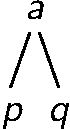
\includegraphics[width=1.17506231142595cm,height=2.17357011675194cm]{functional-lecture05-via-latex-1.pdf}}\hspace{-0.015282697100879cm}$
  &  &
  $\hspace{-0.00839564475928112cm}\raisebox{-0.787418443180629\height}{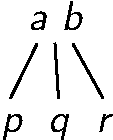
\includegraphics[width=1.90515545061cm,height=2.34987865669684cm]{functional-lecture05-via-latex-2.pdf}}\hspace{-0.0624426078971534cm}$
  &  &
  $\hspace{-0.00839564475928112cm}\raisebox{-0.787418443180629\height}{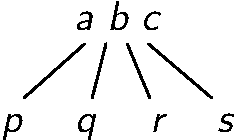
\includegraphics[width=3.94687131050767cm,height=2.34987865669684cm]{functional-lecture05-via-latex-3.pdf}}\hspace{-0.0384199134199137cm}$\\
  2-node &  & 3-node &  & 4-node
\end{tabular}}}

To insert ``25'' into (``.'' stand for leaves, ignored later)
\[ 
   \raisebox{-0.879772896906266\height}{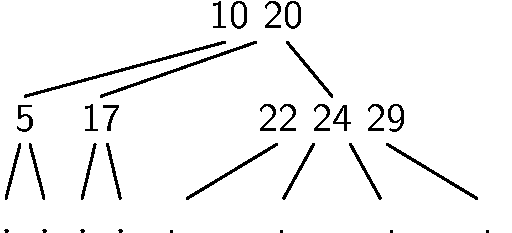
\includegraphics[width=8.5959595959596cm,height=3.91056670602125cm]{functional-lecture05-via-latex-4.pdf}}
\]
we descend right, but it is a full node, so we move the middle up and split
the remaining elements:
\[ 
   \raisebox{-0.787389605285599\height}{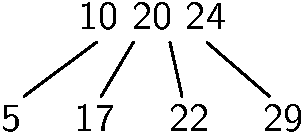
\includegraphics[width=5.0965663124754cm,height=2.2113505181687cm]{functional-lecture05-via-latex-5.pdf}}
\]
Now there is a place between 24 and 29: next to 29
\[ 
   \raisebox{-0.787389605285599\height}{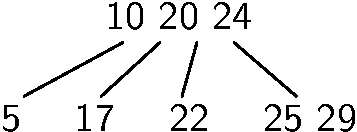
\includegraphics[width=5.99962285189558cm,height=2.2113505181687cm]{functional-lecture05-via-latex-6.pdf}}
\]


To represent 2-3-4 tree as a binary tree with one element per node, we color
the middle element of a 4-node, or the first element of 2-/3-node, black and
make it the parent of its neighbor elements, and make them parents of the
original subtrees. Turning this:

Red-black\_tree\_B-tree.png

into this Red-Black tree:

Red-black\_tree\_example.png

\subsection{Red-Black trees, without deletion}

\begin{itemize}
  \item {\tmstrong{Invariant 1.}} No red node has a red child.
  
  \item {\tmstrong{Invariant 2}}. Every path from the root to an empty node
  contains the same number of black nodes.
  
  \item First we implement Red-Black tree based sets without deletion.
  
  \item The implementation proceeds almost exactly like for unbalanced binary
  search trees, we only need to restore invariants.
  
  \item By keeping balance at each step of constructing a node, it is enough
  to check locally (around the root of the subtree).
  
  \item For understandable implementation of deletion, we need to introduce
  more colors. See Matt Might's post edited in a separate file.
\end{itemize}


{\small{{\hlkwa{type }}{\hlstd{color }}{\hlopt{= }}{\hlkwd{R
}}{\hlopt{\textbar }}{\hlkwd{B}}{\hlendline{}}\\
{\hlkwa{type }}{\hlstd{'a t }}{\hlopt{= }}{\hlkwd{E }}{\hlopt{\textbar
}}{\hlkwd{T }}{\hlkwa{of }}{\hlstd{color }}{\hlopt{* }}{\hlstd{'a t
}}{\hlopt{* }}{\hlstd{'a }}{\hlopt{* }}{\hlstd{'a t}}{\hlendline{}}\\
{\hlkwa{let }}{\hlstd{empty }}{\hlopt{= }}{\hlkwd{E}}{\hlendline{}}\\
{\hlkwa{let rec }}{\hlstd{member x m }}{\hlopt{=}}{\hlendline{}}\\
{\hlstd{ \ }}{\hlkwa{match }}{\hlstd{m }}{\hlkwa{with}}{\hlendline{Like in
unbalanced binary search tree.}}\\
{\hlstd{ \ }}{\hlopt{\textbar }}{\hlkwd{Empty }}{\hlopt{->
}}{\hlkwa{false}}{\hlendline{}}\\
{\hlstd{ \ }}{\hlopt{\textbar }}{\hlkwd{T
}}{\hlopt{(}}{\hlstd{{\textunderscore}}}{\hlopt{,
}}{\hlstd{{\textunderscore}}}{\hlopt{, }}{\hlstd{y}}{\hlopt{,
}}{\hlstd{{\textunderscore}}}{\hlopt{) }}{\hlkwa{when }}{\hlstd{x }}{\hlopt{=
}}{\hlstd{y }}{\hlopt{-> }}{\hlkwa{true}}{\hlendline{}}\\
{\hlstd{ \ }}{\hlopt{\textbar }}{\hlkwd{T
}}{\hlopt{(}}{\hlstd{{\textunderscore}}}{\hlopt{, }}{\hlstd{a}}{\hlopt{,
}}{\hlstd{y}}{\hlopt{, }}{\hlstd{{\textunderscore}}}{\hlopt{) }}{\hlkwa{when
}}{\hlstd{x }}{\hlopt{< }}{\hlstd{y }}{\hlopt{-> }}{\hlstd{member x
a{\hlendline{}}\\
\ }}{\hlopt{\textbar }}{\hlkwd{T
}}{\hlopt{(}}{\hlstd{{\textunderscore}}}{\hlopt{,
}}{\hlstd{{\textunderscore}}}{\hlopt{, }}{\hlstd{{\textunderscore}}}{\hlopt{,
}}{\hlstd{b}}{\hlopt{) -> }}{\hlstd{member x b}}{\hlendline{}}\\
{\hlkwa{let }}{\hlstd{balance }}{\hlopt{=
}}{\hlkwa{function}}{\hlendline{Restoring the invariants.}}\\
{\hlstd{ \ }}{\hlopt{\textbar }}{\hlkwd{B}}{\hlopt{,}}{\hlkwd{T
}}{\hlopt{(}}{\hlkwd{R}}{\hlopt{,}}{\hlkwd{T
}}{\hlopt{(}}{\hlkwd{R}}{\hlopt{,}}{\hlstd{a}}{\hlopt{,}}{\hlstd{x}}{\hlopt{,}}{\hlstd{b}}{\hlopt{),}}{\hlstd{y}}{\hlopt{,}}{\hlstd{c}}{\hlopt{),}}{\hlstd{z}}{\hlopt{,}}{\hlstd{d}}{\hlendline{On
next figure: left,}}\\
{\hlstd{ \ }}{\hlopt{\textbar }}{\hlkwd{B}}{\hlopt{,}}{\hlkwd{T
}}{\hlopt{(}}{\hlkwd{R}}{\hlopt{,}}{\hlstd{a}}{\hlopt{,}}{\hlstd{x}}{\hlopt{,}}{\hlkwd{T
}}{\hlopt{(}}{\hlkwd{R}}{\hlopt{,}}{\hlstd{b}}{\hlopt{,}}{\hlstd{y}}{\hlopt{,}}{\hlstd{c}}{\hlopt{)),}}{\hlstd{z}}{\hlopt{,}}{\hlstd{d{\hlendline{top,}}\\
\ }}{\hlopt{\textbar
}}{\hlkwd{B}}{\hlopt{,}}{\hlstd{a}}{\hlopt{,}}{\hlstd{x}}{\hlopt{,}}{\hlkwd{T
}}{\hlopt{(}}{\hlkwd{R}}{\hlopt{,}}{\hlkwd{T
}}{\hlopt{(}}{\hlkwd{R}}{\hlopt{,}}{\hlstd{b}}{\hlopt{,}}{\hlstd{y}}{\hlopt{,}}{\hlstd{c}}{\hlopt{),}}{\hlstd{z}}{\hlopt{,}}{\hlstd{d}}{\hlopt{)}}{\hlendline{bottom,}}\\
{\hlstd{ \ }}{\hlopt{\textbar
}}{\hlkwd{B}}{\hlopt{,}}{\hlstd{a}}{\hlopt{,}}{\hlstd{x}}{\hlopt{,}}{\hlkwd{T
}}{\hlopt{(}}{\hlkwd{R}}{\hlopt{,}}{\hlstd{b}}{\hlopt{,}}{\hlstd{y}}{\hlopt{,}}{\hlkwd{T
}}{\hlopt{(}}{\hlkwd{R}}{\hlopt{,}}{\hlstd{c}}{\hlopt{,}}{\hlstd{z}}{\hlopt{,}}{\hlstd{d}}{\hlopt{))}}{\hlendline{right,}}\\
{\hlstd{ \ \ \ }}{\hlopt{-> }}{\hlkwd{T
}}{\hlopt{(}}{\hlkwd{R}}{\hlopt{,}}{\hlkwd{T
}}{\hlopt{(}}{\hlkwd{B}}{\hlopt{,}}{\hlstd{a}}{\hlopt{,}}{\hlstd{x}}{\hlopt{,}}{\hlstd{b}}{\hlopt{),}}{\hlstd{y}}{\hlopt{,}}{\hlkwd{T
}}{\hlopt{(}}{\hlkwd{B}}{\hlopt{,}}{\hlstd{c}}{\hlopt{,}}{\hlstd{z}}{\hlopt{,}}{\hlstd{d}}{\hlopt{))}}{\hlendline{center
tree.}}\\
{\hlstd{ \ {\hlopt{\textbar}}
color}}{\hlopt{,}}{\hlstd{a}}{\hlopt{,}}{\hlstd{x}}{\hlopt{,}}{\hlstd{b
}}{\hlopt{-> }}{\hlkwd{T
}}{\hlopt{(}}{\hlstd{color}}{\hlopt{,}}{\hlstd{a}}{\hlopt{,}}{\hlstd{x}}{\hlopt{,}}{\hlstd{b}}{\hlopt{)}}{\hlendline{We
allow red-red violation for now.}}{\newpage}

{\hlkwa{let }}{\hlstd{insert x s }}{\hlopt{=}}{\hlendline{}}\\
{\hlstd{ \ }}{\hlkwa{let rec }}{\hlstd{ins }}{\hlopt{=
}}{\hlkwa{function}}{\hlendline{Like in unbalanced binary search tree,}}\\
{\hlstd{ \ \ \ }}{\hlopt{\textbar }}{\hlkwd{E }}{\hlopt{-> }}{\hlkwd{T
}}{\hlopt{(}}{\hlkwd{R}}{\hlopt{,}}{\hlkwd{E}}{\hlopt{,}}{\hlstd{x}}{\hlopt{,}}{\hlkwd{E}}{\hlopt{)}}{\hlendline{but
fix violation above created node.}}\\
{\hlstd{ \ \ \ }}{\hlopt{\textbar }}{\hlkwd{T
}}{\hlopt{(}}{\hlstd{color}}{\hlopt{,}}{\hlstd{a}}{\hlopt{,}}{\hlstd{y}}{\hlopt{,}}{\hlstd{b}}{\hlopt{)
}}{\hlkwa{as }}{\hlstd{s }}{\hlopt{->}}{\hlendline{}}\\
{\hlstd{ \ \ \ \ \ }}{\hlkwa{if }}{\hlstd{x}}{\hlopt{<}}{\hlstd{y
}}{\hlkwa{then }}{\hlstd{balance
}}{\hlopt{(}}{\hlstd{color}}{\hlopt{,}}{\hlstd{ins
a}}{\hlopt{,}}{\hlstd{y}}{\hlopt{,}}{\hlstd{b}}{\hlopt{)}}{\hlendline{}}\\
{\hlstd{ \ \ \ \ \ }}{\hlkwa{else if }}{\hlstd{x}}{\hlopt{>}}{\hlstd{y
}}{\hlkwa{then }}{\hlstd{balance
}}{\hlopt{(}}{\hlstd{color}}{\hlopt{,}}{\hlstd{a}}{\hlopt{,}}{\hlstd{y}}{\hlopt{,}}{\hlstd{ins
b}}{\hlopt{)}}{\hlendline{}}\\
{\hlstd{ \ \ \ \ \ }}{\hlkwa{else }}{\hlstd{s }}{\hlkwa{in}}{\hlendline{}}\\
{\hlstd{ \ }}{\hlkwa{match }}{\hlstd{ins s }}{\hlkwa{with}}{\hlendline{We
could still have red-red violation at root,}}\\
{\hlstd{ \ }}{\hlopt{\textbar }}{\hlkwd{T
}}{\hlopt{(}}{\hlstd{{\textunderscore}}}{\hlopt{,}}{\hlstd{a}}{\hlopt{,}}{\hlstd{y}}{\hlopt{,}}{\hlstd{b}}{\hlopt{)
-> }}{\hlkwd{T
}}{\hlopt{(}}{\hlkwd{B}}{\hlopt{,}}{\hlstd{a}}{\hlopt{,}}{\hlstd{y}}{\hlopt{,}}{\hlstd{b}}{\hlopt{)}}{\hlendline{fixed
by coloring it black.}}\\
{\hlstd{ \ }}{\hlopt{\textbar }}{\hlkwd{E }}{\hlopt{-> }}{\hlstd{failwith
}}{\hlstr{"insert: impossible"}}{\hlendline{}}}}

\

{\small{\begin{tabular}{lll}
  {\hlkwd{B}}{\hlopt{,}}{\hlkwd{T }}{\hlopt{(}}{\hlkwd{R}}{\hlopt{,}}{\hlkwd{T
  }}{\hlopt{(}}{\hlkwd{R}}{\hlopt{,}}{\hlstd{a}}{\hlopt{,}}{\hlstd{x}}{\hlopt{,}}{\hlstd{b}}{\hlopt{),}}{\hlstd{y}}{\hlopt{,}}{\hlstd{c}}{\hlopt{),}}{\hlstd{z}}{\hlopt{,}}{\hlstd{d}}
  &
  $\underset{\Downarrow}{\hspace{-0.00839564475928112cm}\raisebox{-0.94114749252849\height}{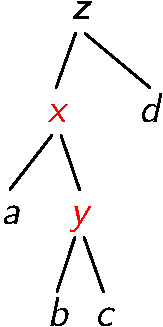
\includegraphics[width=2.7423914469369cm,height=5.49224386724387cm]{functional-lecture05-via-latex-7.pdf}}\hspace{-0.0530630985176441cm}}$
  & {\hlkwd{B}}{\hlopt{,}}{\hlkwd{T
  }}{\hlopt{(}}{\hlkwd{R}}{\hlopt{,}}{\hlstd{a}}{\hlopt{,}}{\hlstd{x}}{\hlopt{,}}{\hlkwd{T
  }}{\hlopt{(}}{\hlkwd{R}}{\hlopt{,}}{\hlstd{b}}{\hlopt{,}}{\hlstd{y}}{\hlopt{,}}{\hlstd{c}}{\hlopt{)),}}{\hlstd{z}}{\hlopt{,}}{\hlstd{d}}\\
  $\hspace{-0.00839564475928112cm}\raisebox{-0.94114749252849\height}{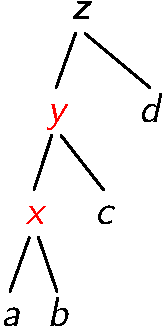
\includegraphics[width=2.7423914469369cm,height=5.49224386724387cm]{functional-lecture05-via-latex-8.pdf}}\hspace{-0.0530630985176441cm}
  \Rightarrow$ &
  $\hspace{-0.00839564475928112cm}\raisebox{-0.917463249710267\height}{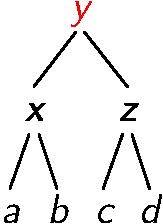
\includegraphics[width=2.7423914469369cm,height=3.76364292273383cm]{functional-lecture05-via-latex-9.pdf}}\hspace{-0.0530630985176441cm}$
  & $\Leftarrow
  \hspace{-0.00839564475928112cm}\raisebox{-0.941102476074375\height}{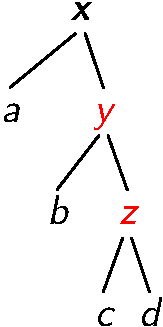
\includegraphics[width=2.7423914469369cm,height=5.48804604486423cm]{functional-lecture05-via-latex-10.pdf}}\hspace{-0.0530630985176441cm}$\\
  {\hlkwd{B}}{\hlopt{,}}{\hlstd{a}}{\hlopt{,}}{\hlstd{x}}{\hlopt{,}}{\hlkwd{T
  }}{\hlopt{(}}{\hlkwd{R}}{\hlopt{,}}{\hlkwd{T
  }}{\hlopt{(}}{\hlkwd{R}}{\hlopt{,}}{\hlstd{b}}{\hlopt{,}}{\hlstd{y}}{\hlopt{,}}{\hlstd{c}}{\hlopt{),}}{\hlstd{z}}{\hlopt{,}}{\hlstd{d}}{\hlopt{)}}
  &
  $\overset{\Uparrow}{\hspace{-0.00839564475928112cm}\raisebox{-0.94114749252849\height}{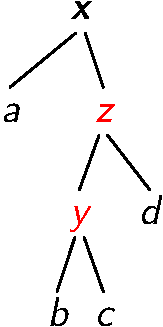
\includegraphics[width=2.7423914469369cm,height=5.49224386724387cm]{functional-lecture05-via-latex-11.pdf}}\hspace{-0.0530630985176441cm}}$
  &
  {\hlkwd{B}}{\hlopt{,}}{\hlstd{a}}{\hlopt{,}}{\hlstd{x}}{\hlopt{,}}{\hlkwd{T
  }}{\hlopt{(}}{\hlkwd{R}}{\hlopt{,}}{\hlstd{b}}{\hlopt{,}}{\hlstd{y}}{\hlopt{,}}{\hlkwd{T
  }}{\hlopt{(}}{\hlkwd{R}}{\hlopt{,}}{\hlstd{c}}{\hlopt{,}}{\hlstd{z}}{\hlopt{,}}{\hlstd{d}}{\hlopt{))}}
\end{tabular}}}

\

\section{Homework}

\begin{enumerate}
  \item Derive the equations and solve them to find the type for:
  
  {\hlkwa{let }}{\hlstd{cadr l }}{\hlopt{=
  }}{\hlkwc{List}}{\hlopt{.}}{\hlstd{hd
  }}{\hlopt{(}}{\hlkwc{List}}{\hlopt{.}}{\hlstd{tl l}}{\hlopt{) }}{\hlkwa{in
  }}\\
  {\hlstd{cadr }}{\hlopt{(}}{\hlnum{1}}{\hlopt{::}}{\hlnum{2}}{\hlopt{::[]),
  }}{\hlstd{cadr
  }}{\hlopt{(}}{\hlkwa{true}}{\hlopt{::}}{\hlkwa{false}}{\hlopt{::[])}}
  
  in environ. $\Gamma = \left\{ \text{{\hlkwc{List}}{\hlopt{.}}{\hlstd{hd}}} :
  \forall \alpha . \alpha \tmop{list} \rightarrow \alpha ;
  \text{{\hlkwc{List}}{\hlopt{.}}{\hlstd{tl}}} : \forall \alpha . \alpha
  \tmop{list} \rightarrow \alpha \tmop{list} \right\}$. You can take
  ``shortcuts'' if it is too many equations to write down.
  
  \item What does it mean that an implementation has junk (as an algebraic
  structure for a given signature)? Is it bad?
  
  \item Define a monomorphic algebraic specification (other than, but similar
  to, $\tmop{nat}_p$ or $\tmop{string}_p$, some useful data type).
  
  \item Discuss an example of a (monomorphic) algebraic specification where it
  would be useful to drop some axioms (giving up monomorphicity) to allow more
  efficient implementations.
  
  \item Does the example {\hlkwc{ListMap}} meet the requirements of the
  algebraic specification for maps? Hint: here is the definition of
  {\hlkwc{List}}{\hlopt{.}}{\hlstd{remove{\textunderscore}assoc}};
  \tmverbatim{compare a x} equals {\hlnum{0}} if and only if
  \tmverbatim{a}{\hlopt{ = }}\tmverbatim{x}.
  
  {\small{{\hlkwa{let rec }}{\hlstd{remove{\textunderscore}assoc x }}{\hlopt{=
  }}{\hlkwa{function}}{\hlendline{}}\\
  {\hlstd{ \ }}{\hlopt{\textbar  [] -> []}}{\hlendline{}}\\
  {\hlstd{ \ }}{\hlopt{\textbar  (}}{\hlstd{a}}{\hlopt{, }}{\hlstd{b
  }}{\hlkwa{as }}{\hlstd{pair}}{\hlopt{) :: }}{\hlstd{l
  }}{\hlopt{->}}{\hlendline{}}\\
  {\hlstd{ \ \ \ \ \ }}{\hlkwa{if }}{\hlstd{compare a x }}{\hlopt{=
  }}{\hlnum{0 }}{\hlkwa{then }}{\hlstd{l }}{\hlkwa{else }}{\hlstd{pair
  }}{\hlopt{:: }}{\hlstd{remove{\textunderscore}assoc x l}}{\hlendline{}}}}
  
  \item Trick question: what is the computational complexity of
  {\hlkwc{ListMap}} or {\hlkwc{TrivialMap}}?
  
  \item * The implementation {\hlkwc{MyListMap}} is inefficient: it performs a
  lot of copying and is not tail-recursive. Optimize it (without changing the
  type definition).
  
  \item Add (and specify) $\tmop{isEmpty} : (\alpha, \beta) \tmop{map}
  \rightarrow \tmop{bool}$ to the example algebraic specification of maps
  without increasing the burden on its implementations (i.e. without affecting
  implementations of other operations). Hint: equational reasoning might be
  not enough; consider an equivalence relation $\approx$ meaning ``have the
  same keys'', defined and used just in the axioms of the specification.
  
  \item Design an algebraic specification and write a signature for
  first-in-first-out queues. Provide two implementations: one straightforward
  using a list, and another one using two lists: one for freshly added
  elements providing efficient queueing of new elements, and ``reversed'' one
  for efficient popping of old elements.
  
  \item Design an algebraic specification and write a signature for sets.
  Provide two implementations: one straightforward using a list, and another
  one using a map into the unit type.
  
  \item (Ex. 2.2 in Chris Okasaki ``Purely Functional Data Structures'') In
  the worst case, \tmverbatim{member} performs approximately $2 d$
  comparisons, where $d$ is the depth of the tree. Rewrite \tmverbatim{member}
  to take no mare than $d + 1$ comparisons by keeping track of a candidate
  element that {\tmem{might}} be equal to the query element (say, the last
  element for which $<$ returned false) and checking for equality only when
  you hit the bottom of the tree.
  
  \item (Ex. 3.10 in Chris Okasaki ``Purely Functional Data Structures'') The
  \tmverbatim{balance} function currently performs several unnecessary tests:
  when e.g. \tmverbatim{ins} recurses on the left child, there are no
  violations on the right child.
  \begin{enumerate}
    \item Split \tmverbatim{balance} into \tmverbatim{lbalance} and
    \tmverbatim{rbalance} that test for violations of left resp. right child
    only. Replace calls to \tmverbatim{balance} appropriately.
    
    \item One of the remaining tests on grandchildren is also unnecessary.
    Rewrite \tmverbatim{ins} so that it never tests the color of nodes not on
    the search path.
  \end{enumerate}
  \item * Implement maps (i.e. write a module for the map signature) based on
  AVL trees. See \tmverbatim{http://en.wikipedia.org/wiki/AVL\_tree}.
\end{enumerate}

\end{document}
